\documentclass[preprint,9pt]{sigplanconf}
\usepackage{url}
\usepackage{listings}
\usepackage{subfigure}
\usepackage{times}
\usepackage{multirow}
\usepackage{color}
\usepackage{multicol}
\usepackage{amsmath}
\usepackage{amssymb}
\usepackage{setspace}
\usepackage{graphicx}
\usepackage{xspace}
\usepackage{color}
\usepackage{rotating}

\newcommand{\addtodo}[1]{\textcolor{red}{[To do: #1]}}
\newcommand{\ctrap}{CTrap\xspace}
\newcommand{\ctraps}{CTraps\xspace}
\newcommand{\ctrapsfull}{CTraps-Full\xspace}
\newcommand{\ctrapsmm}{CTraps-NRR\xspace}
\newcommand{\lws}{CTraps-LWS\xspace}
\newcommand{\lwt}{LWT\xspace}


\newcommand{\Caption}[1]{\begin{minipage}{1.0\columnwidth} \caption{#1} \end{minipage}\vspace{-2ex}}
\newcommand{\CaptionWide}[1]{\caption{#1}\vspace{-2ex}}
%\doublespacing
\authorinfo{Anonymous for Submission}{}

\title{\Large Last Writer Slices and Communication Traps}

%\authorinfo{Brandon Lucia \and Luis Ceze}{University of Washington, Department of Computer Science and Engineering}{\{blucia0a,luisceze\}@cs.washington.edu\\http://sampa.cs.washington.edu\\{\bf In Submission --- Please Do Not Distribute}}

%\author{Anonymous for Submission}
\begin{document}
\maketitle

\begin{abstract}
%Monitoring inter-thread memory dependences in production is useful.  Doing so
%improves debugging information and provides information to dynamic analyses and
%runtime systems.  Prior work that continuously monitors cross-thread
%dependences typically has overheads too high for production.  

We design efficient system support for collecting {\em last writer slices} for
shared-memory concurrent programs.  Last writer slices dynamically track memory
updates.  Last writer slices encode the provenance of values in memory, helping
with debugging.   We build on last writer slices, developing {\em communication
traps} (\ctraps).  \ctraps uses system support to efficiently monitor and
interpose on inter-thread memory dependences.  \ctraps provides an extensible
framework, exposing inter-thread dependences to {\em \ctraps applications}.
These can implement arbitrary dependence analyses.  

We implement last writer slicing and \ctraps.  We show \ctraps is useful by
implementing two applications from prior work. We show that last writer slices
help with debugging using case studies of real-world bugs.  We evaluate our
designs on a set of server programs and standard benchmarks.  Our results show
\ctraps imposes overheads low enough for use in production systems (0--15\%)
running important services, like memcached, LevelDB, MySQL, and Apache.

\end{abstract}

\section{Introduction}
Multi-threaded programming is challenging.  In contrast to the simplicity of
sequential reasoning, multi-threaded programs require complex reasoning about
many threads of control and their interactions.  In shared memory programs,
threads interact by reading and writing memory locations.  Threads' reads and
writes interleave arbitrarily and nondeterministically, with each interleaving
potentially yielding different execution behavior.  The complexity of reasoning
about thread interactions is a central challenge to building multi-threaded
software.  

When programmers reason incorrectly, they permit some interleavings that should
be forbidden.  When such interleavings occur, program executions may fail,
experience performance degradation, or suffer other undesirable behavior.
Preventing such undesirable behavior is a fundamental challenge faced by
software engineers.  One important way to understand program behavior is to
monitor which read and write operations {\em depend} on one another.  Memory
operations are dependent if their order determines the values they read or
write.  Dependences are especially useful for understanding how threads
interact.   


%\cite{defuse,conseq,recon,bugaboo,raceslicing,fasttrack,falcon}
%\cite{oshajava,osha} 
%\cite{avio,dmtracker,cci,daikon}
%\cite{aviso,cfix} 
%\cite{mtperf,criticalitypredictors,schedpredictionmodel}  
%\cite{defuse}
%\cite{avio,cci,defuse,recon,bugaboo,falcon,dmtracker,aviso,cfix,criticalitypredictors,schedpredictionmodel}

Prior work has used dependence information to reduce the burden of making
reliable, efficient concurrent software.  Bug
detection~\cite{avio,fasttrack,raceslicing,dmtracker} and
debugging~\cite{tipslicingsurvey,bugaboo,recon,cci,defuse,conseq,falcon} tools
analyze inter-thread dependences to find buggy behavior and help programmers
understand their errors.
Profilers~\cite{threadclustering,schedpredictionmodel} analyze inter-thread
dependences to find optimization opportunities.  Dependences are also essential
to some program understanding systems~\cite{oshatr} and dynamic checkers for
thread interaction properties~\cite{oshajava,velodrome}.
Record-Replay~\cite{chimera,doubleplay,fdr,rtr} systems track and record the
order of dependent events to help reproduce failures.  

%Deterministic execution
%systems~\cite{coredet,grace} monitor dependences to determine how and when to
%serialize portions of threads' executions to enforce determinism.  Software
%trasactional memory (STM) systems~\cite{stm} monitor dependences to identify
%conflicts between concurrently executing atomic code regions.  

We note that monitoring dependences is not only a fundamental part of the value
of such systems, but also a fundamental part of the {\em cost}.  Tracking
dependences requires executing additional monitoring code while the program
runs and many of the above systems have reported overheads too high for use in
production (10-100x
slowdown)~\cite{raceslicing,dmtracker,velodrome,recon,defuse,oshajava,chimera,coredet,stm}.
Unfortunately, many of these systems are most effective when they run in
production.

We argue in this work that dependence-tracking analysis should -- and can --
have low enough overhead for use in deployed systems.  The key to reducing the
overhead of dependence tracking is to carefully select and monitor only a
{\em subset} of dependences.  We start from two simple observations: (1) Reads are
frequent so we must minimize tracking overheads on reads, and (2) When
addressing concurrency, {\em inter-thread} dependences are most important.
Based on these observations, we focus on dependences that reflect {\em
communication} between threads.  Communication occurs when a thread reads or
overwrites a memory location that was most recently written by a different
thread; {\em i.e.}, inter-thread read-after-write (RAW) and write-after-write
(WAW).  Tracking only communication dependences preserves enough information to
implement useful applications, but has low enough overhead for always-on use in
production.  Framed by this idea, there are two parts to our work.

First, we describe {\em last writer slices}
(Section~\ref{sec:lastwriterslices}).  Last writer slices record the thread and
program point that last wrote each memory location.  Last writer slices are
useful because they expose the {\em provenance} of a memory location's contents
during debugging (Section~\ref{sec:debugging}).  When a failure occurs, last
writer slices are saved with a core dump.  Last writer slices are also
available during an execution in the debugger.  Tracking last writer slices has
low overhead because it only imposes overhead on write operations:  reads are
overhead-free.  In Section~\ref{sec:eval} we experimentally show
that collecting last writer slices has low overhead.

Second, on top of last writer slices we build {\em Communication Traps} or {\em
\ctraps}  (Section~\ref{sec:ctraps}).  \ctraps monitors inter-thread
communication with overhead low enough for production use in many important
cases.  When threads communicate, \ctraps delivers a {\em trap} that can be
handled by a trap handler.  Trap handlers implement {\em \ctraps applications}
through an extensible interface that can analyze or interpose on the execution
(Section~\ref{sec:apps}).  By default, \ctraps has very low overhead.  \ctraps
applications can perform arbitrary dependence analyses, but at their own
discretion and cost.  As we show in our evaluation, the overhead of \ctraps
applications scales with the complexity of their analysis.

\paragraph{Contributions of This Work}
To summarize, this work makes several contributions:
\begin{itemize}

\item{We discuss last-writer slices, an abstraction that dynamically tracks
memory updates, capturing inter-thread dependence information.  We
design and implement system support for collecting last writer slices.  We
present two cases studies that show that last writer slices are useful for
diagnosing real-world bugs.}

\item{Building on last-writer slices, we describe and implement \ctraps, which
exposes inter-thread communication through an extensible trap interface.
We also look at an optimization to \ctraps that explores trading off
precision for performance.}

\item{We demonstrate that \ctraps provides a simple platform for building
dependence analyses by implementing two analyses from prior
work~\cite{cci,defuse,recon}. }

\item{We implement last writer slicing and \ctraps and evaluate their performance using a
variety of important applications ({\em e.g.}, MySQL, memcached and the PARSEC
benchmarks~\cite{parsec}).  We show that in many cases our designs have overheads
low enough for use in deployment (0--15\%).}

\end{itemize}




%In this work, we begin by showing that the cost of monitoring communication has
%been overstated in prior work.  We do so by designing support to monitor
%communication that, for a variety of important applications ({\em
%e.g.},databases, key-value stores, web servers) the overheads are extremely low
%-- so low that communication tracking is viable even for today's deployed
%systems.  We illustrate our claim with system support for  {\em Communication
%Traps} or \ctraps.  Our support for \ctraps tracks communication between
%threads and exposes communication events to trap handlers that can implement
%applications, such as the above.  We show the feasibility of our approach by
%implementing a selection of the above applications, as well as several novel
%applications.  We study the performance characteristics of \ctraps and provide
%a comparison to prior work, showing that our system has lower performance
%overheads -- in some cases, by one to two orders of magnitude lower.  We then
%show that even in cases that, for \ctraps, incur higher performance overheads,
%judicious use of sampling reduces overheads to an acceptable level, and retains
%many of the benefits of non-sampling \ctraps.


\section{Background}

Many systems that support programming and execution models, debugging tools,
and other software engineering tools track dynamic memory dependences during a
program's execution.  In this section we provide context for \ctraps by
discussing some of these systems, focusing on those that address concurrency.
We then briefly discuss debugging with data dependence information, in order to
motivate the role of last writer slices at debugging time.

\subsection{Tracking Dependences and Communication}
\label{sec:background:comm}
%\ctraps tracks dependences that correspond to {\em inter-thread communication}.

A good first example of a system that monitors inter-thread dependences is
software transactional memory (STM)~\cite{stm}.  In STMs, dependences
correspond to interference between accesses in different threads that must be
detected to rollback conflicting transactions.  Deterministic concurrent
runtime systems~\cite{coredet,grace} are similar -- they monitor
inter-thread dependences, to determine when to apply deterministic ordering
constraints on threads' accesses.  STMs and deterministic systems must track
all dependences and they must track them precisely, to provide strong
guarantees as programming and execution models.  Unfortunately, precision can
have a high runtime overhead -- {\em e.g.}, CoreDet incurs a mean overhead of
around 5x~\cite{coredet}.  This overhead is too high for most production
systems.  

%The overhead comes from the need to precisely track read-after-write (RAW),
%write-after-read (WAR), and write-after-write (WAW) dependences, taking action
%({\em e.g.}, buffering) on most cross-thread dependences.  These systems track
%dependences with additional code that runs around memory accesses.  To ensure
%correctness, accesses and tracking code usually must be protected by
%synchronization.  The high cost of synchronization exacerbates the overheads.

In contrast to {\em imprecision intolerant} tasks like STM and deterministic
execution, other tasks are more {\em imprecision tolerant}.  Imprecision
tolerant systems help perform tasks like
debugging~\cite{defuse,conseq,recon,bugaboo,raceslicing,fasttrack,falcon},
software engineering~\cite{oshajava,oshatr}, anomaly
detection~\cite{avio,dmtracker,cci,daikon}, bug and failure
avoidance~\cite{aviso,cfix} and concurrent performance
profiling~\cite{threadcriticality,schedpredictionmodel}.  These
systems also work by monitoring how data flows between threads.  They can
tolerate two important sources of imprecision.

First, many of these techniques track only an {\em ad hoc} subset of
dependences.  For example, DefUse~\cite{defuse} tracks inter-thread WAR
dependences, but not WAW dependences.  Recon tracks some inter-thread WAW and
RAW dependences and approximates WAR dependences.  These techniques are useful
despite an incomplete set of dependences.  Second, many of these systems rely
on statistical models of software
behavior~\cite{avio,cci,defuse,recon,bugaboo,falcon,dmtracker,aviso,threadcriticality,schedpredictionmodel}.
Models often tolerate noise, so many of these techniques can relax the
correctness constraints of their implementation and remain useful.  For
example, some systems have chosen not to enforce atomicity of each memory
access and its dependence tracking code, compromising precision for a boost in
performance.

These tools and techniques work in a variety of environments.  A common theme
is the advantage reaped from use in a deployment environment.  Debugging tools,
profilers, and anomaly detectors benefit from seeing diverse, real-world
behavior.  Dynamic failure avoidance techniques must work in deployed systems
to be effective.  Deployment environments demand low overheads.  

In this work, we select a subset of inter-thread dependences in a systematic
way, rather than choosing an {\em ad hoc} subset.  \ctraps tracks dependences
that correspond to inter-thread communication.  \ctraps provides enough
precision to build useful analyses and runtime systems with overhead low enough
for use in production.


\subsection{Debugging with Data Dependence Information}

Data dependence information is directly useful during program debugging.  A
wide variety of dynamic program slicing
techniques~\cite{thinslicing,tipslicingsurvey} have been proposed.  These
techniques record a subset (slice) of dynamic program instructions selected
using data and control dependence information.  Dynamic dependence slices
expose the provenance of control- and data-flows in the execution.  Work on
debugging~\cite{whylinechi,whylineicse} in the HCI and Software Engineering
community shows that when programmers debug programs, they benefit from the
ability to directly ask such provenance (``why'') questions of their debugger.  


Dynamic dependence slices are especially useful for debugging if they are
available after a failure has occurred in a deployed system. However, slicing
in deployed systems is uncommon, because deployed systems demand low overheads
and slicing can have high overhead.  Our system provides provenance information
that is useful at debugging time by collecting {\em last writer slices} that
help understand inter-thread communication.  We track last writer slices
with overhead low enough for use in production code.  Deployable efficiency
makes it possible to collect and report last writer slices the same way today's
systems collect and report core dumps.

\section{Last Writer Slices}
\label{sec:lastwriterslices}

A last writer slice is a record associated with a memory location that stores
the thread and program point that last wrote data to that memory location.  A
last writer slice is a dynamic property of a memory location at a point in a
program's execution.   We formalize last writer slices in
Section~\ref{sec:lwssoundness}. 

We first discuss last writer slices in more depth by describing the design of
our support for collecting them.  The system support consists of a runtime
library and a compiler analysis.  In Section~\ref{sec:debugging} we highlight
the role of last writer slices in debugging and show they help diagnose real
bugs, using case studies.

\subsection{Runtime Support: Maintaining the Last Writer Table}
We gather last writer slices at runtime by maintaining a {\em last writer
table} (\lwt).  The \lwt is a {\em shadow memory} that holds one entry for each
memory address accessed by the program.  Each \lwt entry records the thread and
program point that last wrote to the entry's corresponding memory location.
When a thread performs a write to a memory location, it updates the \lwt by
recording its thread identifier and the program point of its write operation to
the memory location's \lwt entry.  A program point may be an
instruction address, or a call stack.  We use instructions by default, but our
system supports 2-address bounded call-stacks as well.   

Figure~\ref{fig:basicLWT} shows the basic operation of our runtime support.
The right side of the figure shows a program execution with three threads.  On
the left is the \lwt at the point of each access.  There are two key things to
notice.  First, write operations update the \lwt entry of the memory location
they access.  Second, there is no action necessary for read operations.  Making
read operations cheap is key to making the overhead of last writer slicing low
enough for deployment use.

\begin{figure}[h]
\centering
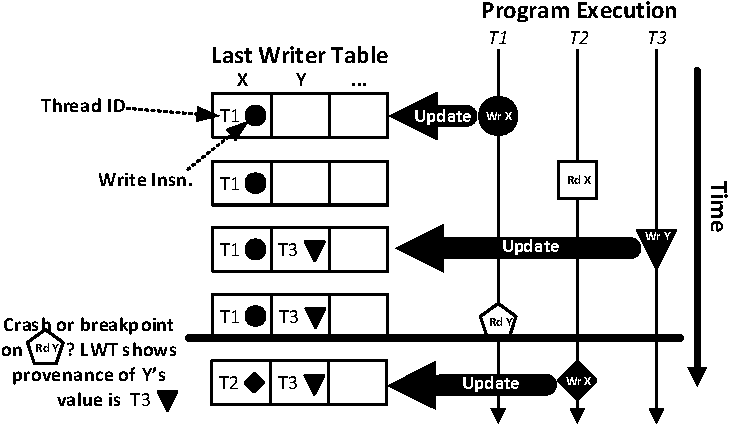
\includegraphics[scale=.6]{figs/BasicLWT.pdf}
\caption{\label{fig:basicLWT}Basic operation of the last writer table. }
\end{figure}

\subsection{Compiler Support: Analysis and Instrumentation}
Collecting last writer slices requires instrumentation on each write operation.
We built an instrumenting compiler pass that inserts a call into our runtime
system just before each write to a memory location that may be accessed by code
executing in another thread (escaping memory accesses).  Write instrumentation
calls are passed three pieces of information: the address of the memory word
involved in the access, the thread identifier of the accessing thread, and the
accessing program point.   

\subsubsection{Escape Analysis}
We use a local function escape analysis to identify which accesses are to
memory locations that can be statically guaranteed to be inaccessible to code
running in other threads.  When a thread accesses a location that is
inaccessible to code in other threads, there is no way that access can be a
communicating access.  Such accesses are not instrumented by our compiler.  

We rely on {\tt GCC}'s built-in escape analysis to determine if a memory
operation might lead to communication.  This analysis is a function escape
analysis.  Locations determined not to escape function scope also cannot escape
the thread executing the function.  However, using an inter-procedural thread
escape analysis may eliminate more instrumentation sites.  Investigating better
instrumentation strategies is orthogonal, but an interesting subject for future
work.

\subsection{Formalism and Correctness}
\label{sec:lwssoundness}
To discuss the correctness of our \lwt-based last writer slice support, we
first develop a formal description of last writer slices.  We consider an
N-threaded program $P = \{P_1, P_2, \ldots P_N\}$, where $P_i = \{p^{i}_{1},
p^{i}_{2}, \ldots, p^{i}_{k_{i}}\}$ is the sequence of $k_{i}$ dynamic
instructions executed by thread $i$.  We assume multi-threaded executions are
sequentially consistent (SC).  Without loss of generality, we assume all
instructions are memory reads and writes, with the form $Op(m)$ where $Op$ is
$Read$ or $Write$. We also assume $m$ is a uniquely addressed memory location.
Under SC, a point in an execution of $P$ after $e$ instructions have
executed is defined by $Q = (q_{0}, \ldots, q_{e})$ where each $q \in Q$ is a
$p^{i}_{j}$ from one of the $k_i$ instructions of thread $i$. We introduce
$LWS[m]$ -- the Last Writer Slice for memory location $m$.   At any point $Q$,
$LWS[m]$ holds $(t,p^{t}_{\ell w})$, where $p^{t}_{\ell w} = max_{\ell}( 
q_{\ell} = Write(m) \in Q)$ and $t$ is the thread that
executed $p^{t}_{\ell w}$. Informally, $p^{t}_{\ell w}$ is the last instruction
in $Q$ to write $m$ and $t$ is the thread that executed it.  For a
never-written location $n$, $LWS[n] = (\emptyset,\emptyset)$ indicating it is
unwritten.

For our design to be correct, $LWT[m]$, the entry for a memory location $m$ in
our \lwt implementation, must be the same as $LWS[m]$ at all points in an
execution.  Correctness in the \lwt requires {\em soundness} and {\em
completeness}.  A {\em sound} design only updates $LWT[m]$ when $m$ is
written.  A {\em complete} design always updates $LWT[m]$ when $m$ is written.
Our compiler inserts \lwt updates before every write
operation (for completeness) and only before write operations (for soundness).
Formally, given a program, $P$, our compiler pass transforms it to a new
program, $P'$.  Each thread in $P'$ executes a modified sequence of
instructions: $P'_{i} \in P' = \{ I(p^{i}_{1}), p^{i}_{1}, \ldots,
I(p^{i}_{k_{i}}), p^{i}_{k_{i}} \}$.  $I(p^{t}_{j})$ sets $LWT[m] =
(t,p^{t}_{j})$ if and only if $p^{t}_{j} = Write(m)$ and is a no-op otherwise.

Thus, our \lwt is correct under the two main assumptions of our formalism: (1)
there are no data races in the execution; and (2) each memory location
referenced by a write refers to a unique region of memory that does not overlap
with another referenced region.  

\paragraph{Sequential Consistency and Data-races}

We assume data-race freedom and a memory model that provides SC under data-race
freedom (implying an SC execution).  We must make these assumptions because,
for performance reasons, we do not enforce the atomicity of \lwt updates and
their corresponding program accesses (a design choice made in prior
work~\cite{fasttrack,recon}).  This atomicity is also required for correctness.    

We use the relation $p \prec q$ to denote that $p$ happens before $q$.  Under
data-race freedom, any write by thread $t$ to $m$, $p^{t}_{j} = Write(m)$,  is
ordered by program synchronization with $p^{t'}_{j'} = Op(m)$, a later access to
$m$ by any other thread $t'$ -- {\em i.e.}, $p^{t}_{j} \prec p^{t'}_{j'}$.  Our
compiler inserts an \lwt update $I(p^{t}_{j})$ into $P'$ before its write
operation, $p^{t}_{j}$, so $I(p^{t}_{j}) \prec p^{t}_{j}$.  Happens-before is
transitive, so $I(p^{t}_{j}) \prec p^{t}_{j} \prec I(p^{t'}_{j'}) \prec
p^{t'}_{j'}$, meaning $I(p^{t}_{j})$ happens before all accesses that
$p^{t}_{j}$ happens before {\em and before their respective \lwt updates},
$I(p^{t'}_{j'})$.  Symmetrically, for any access $p^{t''}_{j''}$ in another
thread $t''$ that precedes $p^{t}_{j}$, $p^{t''}_{j''} \prec p^{t}_{j}$.  Our
compiler inserts each $I(p^{t}_{j})$ immediately before each $p^{t}_{j}$, so
$I(p^{t''}_{j''}) \prec p^{t''}_{j''} \prec I(p^{t}_{j}) \prec p^{t}_{j}$,
happens-before ordering $I(p^{t}_{j})$ after all preceding accesses to $m$ in
other threads, {\em and after their repective \lwt updates}.  Thus, at all
points $Q$ in a data-race free execution, given $q_r = I(p^{t}_{j})$, $q_p =
p^{t}_{j}$, and $q_r \prec q_p$, $\forall_{ \{q_s | q_r \prec q_s \prec q_p
\}}: q_s \ne Op(m) \wedge q_s \ne I(Op(m)) $.  In other words, \lwt updates and
their accesses are atomic.

With data-races, \lwt updates and their accesses may not be atomic ({\em i.e.},
such a $q_s$ can exist).  Instrumentation calls for racy accesses are not
ordered by happens-before, so they may interleave arbitrarily.  With races, an
execution could reach a state $Q_{bad} = (\ldots, I(p^{t}_{j}), I(p^{t'}_{j'}),
p^{t'}_{j'}, p^{t}_{j}, \ldots)$.  In such a state, $LWS[m] = (t,p^{t}_{j})$,
but $LWT[m] = (t',p^{t'}_{j'})$.  The \lwt was effectively not updated when
$p^{t}_{j}$ executed (violating completeness), or was effectively updated to
reflect that $p^{t'}_{j'}$ was $m$'s last writer, when $p^{t}_{j}$ was
(violating soundness).  This edge case is incorrect. However, we expect it is
also uncommon in practice, so last writer slices are usually correct, even in
racy programs.

\paragraph{Non-overlapping Memory References} 
We assume each written memory location corresponds to a non-overlapping memory
region because our \lwt design is {\em granularity oblivious}.  We discuss this
issue only informally due to space constraints.  Each \lwt entry corresponds to
a memory location referenced by a program instruction.  Two instructions might
reference different locations that actually overlap because the referenced
locations have different granularities.  When that happens, both accesses
update different \lwt entries, because they reference different locations.
However, the overlapping region then has two different, inconsistent entries
reflecting its last {\em two} updates, rather than just its last write.

For example, one instruction might write a word and another might later write
the second byte of that word.  The word access updates the word's \lwt entry.
The byte access updates a second \lwt entry for the byte address.  However, the
byte is part of the previously written word, meaning the \lwt entry for the
word no longer reflects reality -- the word was last written by the instruction
and thread that wrote the byte, not the one that wrote the word.  This
situation leads to incompleteness because the entry for the word should be
updated but it is not.

Assuming non-overlapping regions ensures \lwt are correct.  Another
approach would be to assume a fixed \lwt granularity.  We chose our solution
for two reasons.  First, fixing the \lwt at a large granularity ({\em i.e.},
cache-line) precludes sound slicing for fine-grained accesses.  Second, fixing
the \lwt at a small granularity ({\em i.e.}, byte) requires multiple \lwt
updates for larger granularity accesses, increasing overheads.




\subsection{Debugging with Last Writer Slices}
\label{sec:debugging}
Prior work has demonstrated that it is useful during debugging to allow
programmers to ask ``why?'' questions~\cite{whylineicse,whylinechi} about the
provenance of program state.  To answer such questions, prior work has mostly
used dependence slices that include intra-thread
dependences~\cite{whylineicse,conseq,tipslicingsurvey}.  The overhead of
slicing dependence chains and tracking temporal sequences is often high,
relegating such techniques to working on traces~\cite{whylinechi} or debugging
executions.  

The \lwt dynamically records information about write operations -- what thread
and code point last wrote each memory location.   These last writer slices do
not explicitly encode anything about read operations.  However, by looking at
the \lwt at a point in the execution, the provenance of the data being read or
over-written can be determined.  For example, if an assertion failure occurs
due to an erroneous inter-thread data flow, the provenance of the data in the
assertion's condition helps explain why the failure occurred.  Last writer
slices therefore answer an important class of ``why?'' questions related to
concurrency errors.     

Computing last writer slices is fast enough to deploy and use
continuously (see Section~\ref{sec:eval}) and the \lwt can be saved with a core
dump.  Thus last writer slices can (and should) be made part of the standard
debugging information provided when a program fails.  

\subsubsection{Case Studies}

We illustrate the debugging benefits of last writer slices using a set of case
studies.  In each case, we debug a buggy program using last writer slices.  We
show that for some concurrency errors, last writer slices are a good match
because they provide answers to important {\em ``why?''}
questions~\cite{whylineicse}.  

\paragraph{Case Study: PBZip2}
We conducted a case study using a buggy version of PBZip2-0.9.1.    The bug is
a use-after-delete bug that leads to an assertion failure.  A worker thread
tries to acquire a mutex after it has been deleted by the main thread during
shutdown, causing the assertion to fail.  

Last writer slices provide the key piece of information to debug this failure: the last
write to the mutex before the worker tried acquiring it was when the main
thread deleted it.  A developer is likely to begin debugging by checking the
validity of the mutex.  Upon finding it is invalid ({\em
i.e.}, it has been deleted), the developer is likely to probe to determine who 
deleted it.  Without the information in the \lwt, answering that question is difficult
because the main thread may have executed arbitrarily far from where it deleted
the mutex.  With the \lwt, answering that question only requires the developer
to check the mutex's entry.


\paragraph{Case Study: MySQL}
Last writer slices were also useful for debugging a logging system failure in
MySQL-4.0.12.  The bug is an atomicity violation involving two threads.  One
thread rotates the database's log file.  Log rotation involves closing the log
file, marking the log closed, opening a new log file, and marking the log open.
Log rotation should be atomic, but lack of synchronization allows another
thread to run queries during rotation.  The query code checks if the log is
marked closed; if it is not closed, the queries are logged, but if it is
closed, the queries are not logged and the program simply continues.  We added
an assertion to the non-logging case because this behavior is a security
vulnerability.  The bug report describes the bug as ``critical'', so it is
reasonable to assume a programmer that expected all queries to be logged would
write such an assertion after the bug was reported.

We ran the program and concurrently issued a log rotation command, and an
insert query.  The bug manifested ({\em i.e.}, the queries went unlogged) and
our assertion failed, dumping core.  Examining the log's last writer slice in
GDB allowed examining the last thread to mark the log closed.  We discerned it
was the log rotation thread that last marked the log closed during log
rotation.  Knowing how the log ended up marked closed enables reasoning about
what code to change ({\em e.g.}, added synchronization) to prevent the
situation in the future.

While a developer is likely to understand the symptom of the bug (queries go
unlogged) without the information in the \lwt, understanding {\em why} it is marked closed would be
difficult.  This example illustrates how the \lwt fills in the crucial inter-thread
dependence that helps understand why the program failed.



\section{Communication Traps}
\label{sec:ctraps}

\ctraps is a platform for analyzing and interposing on inter-thread
communication events during a concurrent program's execution.  We build our
support for \ctraps on top of the support for last writer slicing that we
described in Section~\ref{sec:lastwriterslices}.  Using last writer slice
information, \ctraps dynamically tracks dependences representing inter-thread
communication events. \ctraps exposes communication events as {\em traps}
during an execution that {\em trap handlers} can handle to perform analysis
and interposition.  We formalize trap delivery and handling in
Section~\ref{sec:ctsoundness}.

\subsection{\ctraps Design}

We now discuss \ctraps in more detail by describing the design of our \ctraps
system support.  Figure~\ref{fig:systemdiagram} shows an overview of our system
support.  The programmer writes their program as usual.  They compile it using
the \ctraps compiler. The \ctraps compiler includes the compiler support for
collecting last writer slices.  In addition, the \ctraps compiler also inserts
calls to the \ctraps runtime at points where communication may occur.  The
resulting compiled executable links to the \ctraps runtime that collects last
writer slices and monitors communication.  The runtime loads and manages \ctraps
handlers when the execution starts via a plugin interface.  \ctraps handlers,
written independently of the original program implement \ctraps applications.
Traps are delivered to handlers by the runtime when operations communicate.
Together, the \ctraps executable and the \ctraps handlers are deployed.


\begin{figure}[htb]
\centering
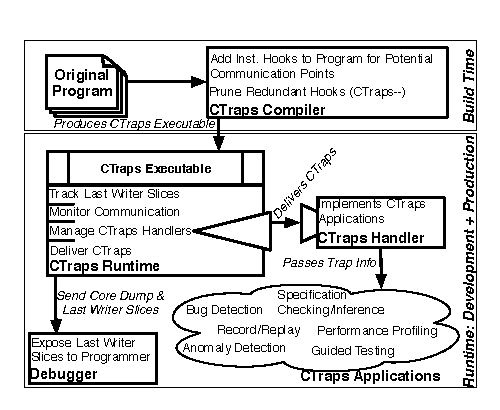
\includegraphics[width=.90\columnwidth]{figs/SystemDiagram.pdf}
\caption{\label{fig:systemdiagram}CTraps system support.}
\end{figure}


%Our system support for \ctraps incorporates the support for collecting last
%writer slices described in Section~\ref{sec:lastwriterslices}.  In addition,
%our \ctraps system support also monitors all read and write operations that
%might communicate and traps on all those that communicate.  
In addition to our base \ctraps design, we also investigate \ctrapsmm, a
variant of \ctraps that uses a flow-sensitive optimization to eliminate some
sources of overhead at a cost in analysis precision. \ctrapsmm tracks all write
operations that might communicate, but leaves some redundant read operations
untracked (\ctraps, with {\bf N}o {\bf R}edundant {\bf R}eads).  

\subsubsection{\ctraps System Support} 

Our base \ctraps design delivers traps on all communicating read and write
operations using compiler and runtime support. 

\paragraph{Compiler Support}
Our compiler instruments all read and write operations that access potentially
escaping memory locations with a call to a {\em trap hook} function.  Trap hooks
are passed the address of the memory word involved in the access, the thread
identifier of the accessing thread, the type of operation being performed, and
the program point of the access.  

\paragraph{Runtime Support}
The \ctraps runtime implements the trap hook function.  Trap hooks have two
purposes: first, to detect communication; second, to deliver traps to \ctraps
applications.  Trap hooks detect communication by looking up the \lwt entry for
the memory location being accessed.  If the thread identifier in the \lwt entry is
different from the accessing thread, then the access is a {\em communicating
memory access}.  At each communicating memory access, the runtime delivers a
trap to the accessing thread just before the memory access is allowed to
proceed.  Traps are delivered by trap hooks to {\em trap handler routines} that
implement \ctraps applications.  Trap handler routines are like signal
handlers.  They are registered with the \ctraps runtime when the program
starts.  Trap handlers may contain arbitrary application-specific code.
Figure~\ref{fig:hookapi} shows the \ctraps trap handling API.  Trap
handlers are passed the four pieces of information passed to the trap hook, as
well as the \lwt's record of the program point and thread identifier of the
last write to the involved memory location.

\begin{figure}[htb]
\centering
\begin{verbatim}
void trap(AccessType type, 
          ThdId currThd, ProgPt currPt,
          ThdId lastThd, ProgPt lastPt);
\end{verbatim}
\caption{\label{fig:hookapi}The \ctraps trap handling interface.}
\end{figure}



\subsubsection{\ctrapsmm: Eliminating Redundant Instrumentation}
\label{sec:dpo}

The runtime support for \ctrapsmm is mostly the same as the runtime support for
our base \ctraps design, but \ctrapsmm adds trap hooks on only a subset of
reads.  \ctrapsmm's compiler support uses the program's control-flow structure
to identify reads that are likely to be {\em redundant}, and eliminates trap
hooks on those accesses.

We use dominator-based analysis to eliminate instrumentation that is likely to
be redundant.  Our analysis is function-local and works on code in SSA form.
The compiler looks at each pair of reads that are instrumented with trap hooks.
If a pair of instrumented reads both refer to a memory address stored in the
same SSA variable and the instrumentation points are {\em control equivalent},
then they are redundant.  Two reads, $A$ and $B$ are control equivalent if $A$
dominates $B$ and $B$ post-dominates $A$ -- every path to $B$ passes through
$A$, and every path passing through $A$ reaches $B$.  The latter read ("$B$")
is not instrumented.  Using this technique to remove instrumentation sites
preserves instrumentation along conditional control flow paths.  For example,
if the second of a pair of reads is conditionally executed, and the first is
not, then the pair are not control equivalent and both remain.  

Figure~\ref{fig:insthooks} illustrates how a pair of control equivalent reads
are instrumented by the compiler for \ctrapsmm.  Pictured on the left is the
original program.  The shapes represent memory accesses with writes marked 'W'
and reads marked 'R'.  Notice that the the pentagon and the diamond are control
equivalent, despite the control flow structure separating them.  Pictured on
the right is the program after instrumentation.  There are two important things
to notice.  First, only the first of the control equivalent accesses are
instrumented, eliminating instrumentation overhead.  Second, the conditionally
executed accesses on either side of the branch are both instrumented.
Preserving these accesses is important for enabling flow-sensitive applications
using \ctrapsmm.  


\begin{figure}[htb]
\centering
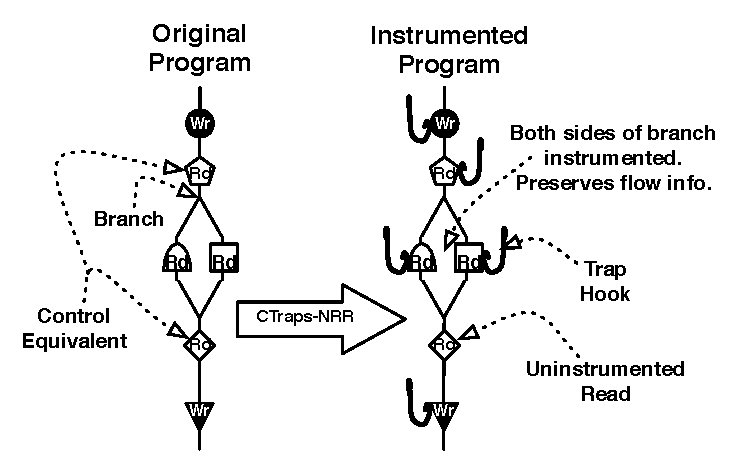
\includegraphics[width=.9\columnwidth]{figs/CTMMHooks.pdf}
\caption{\label{fig:insthooks}Placement of trap hooks for \ctrapsmm.}
\end{figure}

\subsection{Formalism and Correctness}
\label{sec:ctsoundness}
To discuss the correctness of \ctraps, we first formalize trap delivery by
building on our last writer slicing formalism from
Section~\ref{sec:lastwriterslices}.  

Given a program $P'$ already instrumented with \lwt updates, the \ctraps
compiler produces $P''$. A thread $i$ in $P''$ executes a modified instruction
sequence, $P''_{i} = \{ T(p^{i}_{j}), I(p^{i}_{1}), p^{i}_{1},$ $\ldots,
T(p^{i}_{j}), I(p^{i}_{k_{i}}), p^{i}_{k_{i}} \}$, where $T(p^{i}_{j})$ is a
trap hook call.  We consider a point $Q = \{q_1, \ldots, q_{e-2}\}$ after $e-2$
instructions of a sequentially consistent execution have executed and $q_{e} =
p^{i}_{j}$ is about to execute after its trap hook $T(p^{i}_{j})$ and \lwt
update $I(p^{i}_{j})$ execute.  The trap hook $T(p^{i}_{j})$ {\em delivers} a
trap before if $LWT[m] = (t,p^{t}_{\ell w})$ and $i \ne t$.  Informally, the
trap hook delivers a trap before the instruction if the thread that last wrote
$m$ is different from the one executing the instruction.  When a trap hook,
$T(p^{t}_{j})$, delivers a trap, thread $t$ executes an arbitrary trap handler
$H = \{h^{t}_{1}, \ldots, h^{t}_{h_{n}}\}$.  Thus, after the trap, the \lwt
update (if $p^{i}_{j} = Write(m)$), and the instruction execute, the execution
reaches the new point $Q = (q_{1}, \ldots, T(q_{e}), h^{t}_{1}, \ldots,
h^{t}_{h_{n}}, I(q_{e}), q_{e})$, and continues.

We define what makes a \ctraps design sound and complete, and then discuss the
correctness of our design.  A design is {\em sound} if it only delivers a trap
when threads have communicated.  A design is {\em complete} if it always
delivers a trap when threads have communicated.  The \ctraps compiler puts a
trap hook on all read and write operations, and only on those operations.
Assuming a correct \lwt, \ctraps is correct.  The correctness of \ctraps also
relies on data-race freedom and non-overlapping memory references.  The same
arguments for \lwt correctness apply to the correctness of trap delivery and
handling.  Most importantly, data-race freedom implies that trap hooks, \lwt
updates, and accesses are all atomic.


%\paragraph{Escape Analysis}
%All our designs eliminate instrumentation on accesses to memory locations
%statically guaranteed to be inaccessible to other threads.  Doing so has no
%effect on soundness or completeness because accesses to such locations are
%guaranteed never to be communicating.

\paragraph{\ctrapsmm} 

\ctrapsmm has the same soundness guarantees as our base \ctraps design, but
compromises on completeness.  The concession in completeness is the result of
removing instrumentation on redundant reads. 

\ctraps and \ctrapsmm rely on the same \lwt implementation, so all traps
delivered in \ctrapsmm are also delivered in the base \ctraps design.  Hence,
\ctrapsmm has the same soundness guarantee as basic \ctraps.  \ctrapsmm removes
trap hooks on some reads that have trap hooks in our base \ctraps design.
Without trap hooks, \ctrapsmm cannot deliver a trap before these reads, so it
is incomplete.  We designed our redundancy analysis to sacrifice completeness,
but preserve enough trap hooks to remain useful.  In \ctrapsmm, at least one of
each pair of control-equivalent accesses is instrumented with a trap hook.
Preserving at least one instrumenation site per control-equivalent pair
guarantees some monitoring still occurs (although the set of trapping accesses
may decrease substantially compared to our base \ctraps design).  Furthermore,
as Section~\ref{sec:dpo} discusses, instrumentation sites on interesting
control flow paths are preserved under our redundancy analysis.  For many
debugging applications, preserving this control flow information is important.

\subsection{\ctraps Applications}
\label{sec:apps}
\ctraps applications are implemented as shared object plugins ({\em i.e.}, {\tt
.so} files on Linux) that are loaded by our runtime.  They must implement the
\ctraps handler API, which requires a trap handler function and permits a
constructor, destructor,  thread constructor,  thread destructor, which allow
initialization and disposal of global and thread-local state.  A wide variety
of \ctraps applications are possible.  Several such applications were outlined
in Section~\ref{sec:background:comm}.    We implemented two applications, a
version of a debugging analysis from prior work~\cite{cci} and communication
graph collection, similar to that in DefUse~\cite{defuse}, Recon~\cite{recon},
and DMTracker~\cite{dmtracker}.

\paragraph{CCI-Prev Implementation}
CCI-Prev is a technique from CCI~\cite{cci} that computes a set of code points
that access a memory location when the previous access to the same location was
by a different thread.  We implemented a variant of CCI-Prev using \ctraps.  On
communcating read operations, the runtime updates the LWT like it normally does
on writes.  Under this policy, any operation that accesses a location that the
LWT indicates was last accessed by a different thread is recorded.  The set of
recorded accesses is the output of the analysis.  Our \ctraps implementation of
CCI-Prev took about 10 lines of code (on top of our base system). 

\paragraph{Communication Graph Implementation}
Communication graphs are fundamental to several prior debugging
techniques~\cite{recon, bugaboo, defuse}.  We implement simple communication
graph collection using \ctraps.  When a trap is delivered, our implementation records
communication graph edges composed of the code point of the last writer to the
location being accessed and the code point of the trapping access.  The set of
recorded graph edges is the communication graph that we output.  Our \ctraps
implementation of communication graphs took about 50 lines of code (including
output formatting code). 

\paragraph{Other Applications}
In addition to those applications, we envision that a variety of applications
will be enabled by our simple interface.  Anomaly detection and ``likely
invariant'' techniques similar to AVIO~\cite{avio}, Daikon~\cite{daikon}, and
others are a natural fit for \ctraps.  \ctraps provides the support necessary
for implementing specification checkers for specifications related to
inter-thread communication~\cite{velodrome,oshajava}.  Guided testing
tools~\cite{cuzz,chess} and bug detection tools~\cite{ctrigger} focused on
concurrency could also easily implemented as \ctraps applications.  \ctraps
also provides an interesting platform for developing new approaches to
record/replay~\cite{chimera,fdr}.  We expect these and other
applications will become more prevalent with the adoption of \ctraps'
low-overhead, deployable support for communication tracking.

Additionally, \ctraps affords the ability for {\em users} of systems to add
functionality to or extend systems.  This facet seems especially promising for
monitoring or enforcing installation-specific security or performance policies
without the need to modify applications.  While interesting, we relegate such
user-built applications to future work.

%Our redundancy analysis applies only to instrumentation on loads,
%not stores.  Eliminating instrumentation on stores may lead to stale
%information in the \lwt, which could lead to spurious traps.  Eliminating
%reads, on the other hand, can only lead to overlooked communication events,
%never false traps.


%\subsection{Design 3: \lws}
%
%Our final design, \lws, varies the compiler support used by \ctrapsfull and
%\ctrapsmm to simply eliminate instrumentation on all read operations.  With no
%instrumentation on read operations, \lws has the lowest runtime overhead, but
%the most imprecise.  However, despite not collecting information about reads,
%\lws precisely collects last writer slices: all writes are instrumented, so the
%\lwt is a sound, complete reflection of program state.  




%\section{Design Justification}


%We designed \ctraps to satisfy two design goals.
%
%First, our design must be efficient enough to run in useful deployment
%environments without hardware support or sampling.  Second, our design must
%collect enough information at run time to be useful for debugging and to
%facilitate building applications.  
%
%The constraints conflict because deployment use requires minimizing
%instrumentation overheads, but collecting information requires potentially
%high-overhead instrumentation.  Our design was guided by prior work on slicing
%and concurrency debugging, and our empirical assessment of our system
%(Section~\ref{sec:eval}).  The main design challenge is deciding which memory
%dependences to track during the program's execution.  
%
%\paragraph{Tracking Most Dependences with High Overhead} 
%
%At one extreme is a design that captures all RAW, WAW, and WAR dependence
%edges.    
%%Another example is the {\em CCI-Prev} feature 
%%used by CCI~\cite{cci} tracks inter-thread RAW, WAR, WAW, and RAR dependences (and some
%%intra-thread ones) with their {\em CCI-Prev} feature. 
%Such a design collects all dependence information, which is useful for
%debugging and building analysis applications.  However, such a design falls
%short on our efficiency goal. Tracking all dependences requires work on every
%memory operation.  The additional work must update a data structure storing
%dependences and access a thread-shared structure like the \lwt that indicates
%which threads and code points are dependent.  Prior
%work~\cite{stm,coredet,raceslicing} illustrates that the overhead of this
%design point is frequently too high for use in deployment. 
%
%%Tallam, {\em et al} see overheads nearing 1000\% for server
%%programs ({\em e.g.} Apache, MySQL) with largely independent tasks.  Without
%%sampling, CCI's overheads as high as 57,000\% for some applications. In most
%%other cases, overheads are lower, but still too high for deployed use without
%%sampling.  Note that with sampling, CCI has deployable overheads, but we are
%%looking for a deployable design that does not require sampling (Constraint 1).
%
%\paragraph{Tracking Many Dependences with Moderate Overhead}
%Short of tracking all dependences, a system may make the decision to track an
%{\em ad hoc} subset of dependences,  as we discussed in
%Section~\ref{sec:background:comm}.  Such systems work well at their specific task
%({\em e.g.}, debugging a certain class of errors).  They collect enough
%dependence information to be useful for their particular application.  However,
%their usefulness is limited because tracking dependences specific to one
%application does not generalize to new applications.  
%
%One reason for tracking a subset of dependences is to reduce overheads.  Systems
%that track {\em ad hoc} dependences tend to have lower overheads than those
%that track all dependences.
%%DefUse tracks intra- and inter-thread RAR and RAW dependences; Recon tracks
%%inter-thread WAW and WAR dependences, and approximates some other dependences.
%However, these systems mostly fall short of our efficiency goal as well, often having
%overheads greater than 1000\%~\cite{defuse,recon}. Such overheads are too high for deployed
%systems.  Some systems avoid such high overheads, but require hardware
%support~\cite{avio, bugaboo, fdr} or sampling~\cite{cbi,cci} to do so, also
%failing to satisfy our design goal.
%
%\paragraph{CTraps: Tracking Select Dependences with Low Overhead}
%We make the case that our \ctraps designs satisfies our design goals.
%
%The tracking support for \ctraps is built atop last writer slices.  Last writer
%slices require tracking only inter-thread WAW dependences.  Tracking only these
%dependences does not require read operations to be instrumented.   Read
%instrumentation has high overhead because reads are more frequent than writes.
%\lws is efficient because tracking last writer slices does not need to track
%any reads.  The overhead of \ctrapsfull and \ctrapsmm is low by default because
%communication hooks (on reads) are no-ops by default.  \ctraps applications may
%perform more analysis on reads and their performance overhead scales with the
%complexity of their analysis.  We argue that such a ``pay-as-you-go'' model
%that is efficient by default is the right approach, satisfying our efficiency
%design goal.  We carefully evalute the overheads of our systems in
%Section~\ref{sec:eval}.
%
%
%Our \ctraps designs also satisfy our usefulness design goal.  \ctraps is useful for
%implementing analyses, especially those focused on concurrent program behavior.
%Inter-thread communication dependences show how values modified in one thread
%flow to operations in another thread.  This systematically selected subset of
%dependences is general enough for \ctrapsfull and \ctrapsmm to implement
%dynamic analyses related to inter-thread data flow.  Furthermore, with
%overheads low enough for deployement, \ctraps applications are useful not just
%during development, but also at runtime and in production.  \lws is also useful
%for providing important debugging information absent from current systems.  We
%describe the debugging benefits of \lws in in Section~\ref{sec:debugging}.  
%
%%\ctrapsfull and \ctrapsmm provide the ability to track reads, but they remain efficient.  The key to
%%their efficiency is the flexibility of read hooks. By default, the hooks are
%%no-ops.  CTraps {\em applications} can carefully select which dependences to
%%track, potentially increasing overhead with increases in functionality.  The
%%baseline performance of both designs is efficient, satisfying Constraint 1.
%%The flexibility provided by read and write hooks enables a variety of useful
%%applications (two of which we implement and evaluate), satisfying Constraint 2.
%


%\section{Formalism and Correctness}
%\label{sec:soundness}

%We formalize last writer slices and \ctraps.  We then discuss the soundness and
%completeness properties of our last writer slices and \ctraps designs.
%We also discuss the impact on soundness and completeness of eliminating
%redundant read instrumentation in \ctrapsmm.



%\paragraph{Preserving Write Instrumentation}
%Our system does not eliminate any write instrumentation.  Removing
%instrumentation on writes may lead to {\em false traps}.  A false trap occurs
%when a thread executes a memory access, refers to the \lwt, and the \lwt has an
%out-of-date version of the last writer information.  False traps reflect unsoundness.
%
%
%Figure~\ref{fig:unsoundness} illustrates how removing write instrumentation
%leads to unsound trap delivery.  The figure shows memory operations in two
%threads, all of which are assumed instrumented except the triangle marked
%as uninstrumented.  The actual last thread and instruction to write is shown at
%the left alongside the state of the LWT.  The figure assumes the behavior of
%\ctrapsfull, except for the single uninstrumented write operation (all of our
%designs instrument all writes).  The LWT becomes corrupted when Thread 2
%performs its uninstrumented write -- the LWT indicates the last writer was
%Thread 1, but Thread 2's uninstrumented write is the actual last writer.  When
%Thread 2 executes its next read instruction, it refers to the corrupted LWT,
%which indicates the read is communicating.  The system delivers a false trap on
%the read.  This example illustrates the risk of eliminating write
%instrumentation.  Our designs preserve instrumentation on all writes to avoid
%this problematic situation.
%
%\begin{figure}
%\centering
%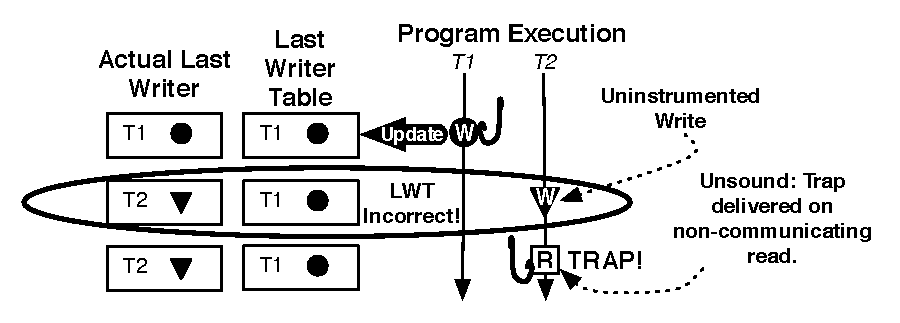
\includegraphics[width=\columnwidth]{figs/unsoundness.pdf}
%\caption{\label{fig:unsoundness}Removing write instrumentation leads to unsoundness.  CTraps does not eliminate instrumentation on writes because it is unsound.}
%\end{figure}
%


%\section{Extensions to \ctraps}
%
%\subsection{Sampling}
%
%\subsection{Context-Sensitivity}


\section{System Implementation and Applications}

We implemented our last writer slicing design, our base \ctraps designs, and
our \ctrapsmm design.  We built our compiler support as a plugin for GCC ({\tt
gcc-4.7.0 20111112}).  We used GCC's points-to and escape analysis support to
prune instrumentation to non-escaping memory locations.  We used GCC's
dominator and post-dominator computations to implement our redundancy analysis.
Our compiler instruments calls to {\tt free} and {\tt delete} as writes to the
pointer being deallocated.  Our analysis handles all code compilable using this
version of GCC except for a few cases: we do not handle accesses that compile
to GCC {\tt BITFIELD\_REFERENCE} IR types because these are undocumented, we do
not handle inlined assembly instructions, and we do not handle C++ exceptions.
Note that these limitations of our research prototype are not fundamental and
the limited cases are uncommon.   

We built our runtime system from scratch in about 1000 lines of C and C++ code.
We implemented the LWT as a fixed size 2GB array of 64-bit words.  Each entry
packs a program point and a thread identifier into the 64-bit word.  By
default, program points are instruction addresses, but we also support bounded
(2-address) context-sensitivity by packing the current instruction's address
and the nearest return address into an LWT entry. When an access to a memory
location occurs, we index into the LWT with the lower bits of the location's
address.  Our prototype implementation uses a lossy resolution policy for hash
collisions.  We use this policy in our prototype because it is faster and
simpler than a chaining concurrent hash table implementation.  Collisions are
extremely rare, so this simplification is unlikely to be a problem even in a
more industrial strength implementation.  




\section{Evaluation}
\label{sec:eval}
We evaluated our design along several axes. Recall that in
Section~\ref{sec:debugging} we illustrated the debugging benefits of last
writer slices using case studies.   We evaluate our performance overheads to
demonstrate that last writer slices and \ctraps are feasible for use in
deployed systems.  We discuss the sources of \ctraps' overhead.   We show that
\ctraps is useful by implementing two existing applications and analyzing their
performance.  We characterize our instrumentation and the precision and
performance impact of our redundancy analysis.  

\subsection{Setup and Benchmarks}

We conducted our evaluation on a machine running Linux 2.6.27-7, with a 2.27GHz
8-core Xeon E5520 processor with 2-way SMT ({\em i.e.}, 16 execution contexts)
and 10GB of memory.  We evaluated \ctraps using PARSEC, a set of architectural
benchmark programs~\cite{parsec} and a collection of real server and desktop
applications.    

\subsubsection{PARSEC}

We ran PARSEC programs with their {\tt native} input set, and with each
program's 8 thread configuration. We have omitted three of the PARSEC
benchmarks because our compiler pass does not handle C++ exceptions.    

\subsubsection{Servers}


\paragraph{MySQL-5.1.65} MySQL is an industrial-strength database
server. To benchmark MySQL, we used {\tt SysBench OLTP} running with its
default 8 threaded configuration, measuring MySQL's performance to be the
throughput reported by {\tt SysBench}.  

\paragraph{Apache-2.4.3} 
Apache-httpd is a popular web server.  To benchmark Apache, we used {\tt
ApacheBench} to request a static {\tt html} page 1,000,000 times using 8 threads,
measuring Apache's performance to be the throughput reported by {\tt
ApacheBench}.  

\paragraph{LevelDB-1.5.0}
LevelDB is a carefully tuned high-performance key-value store written by Google
developers. To benchmark LevelDB, we used the included {\tt db\_bench} utility,
running its ``Read while Writing'' test with 8 threads.  We measure LevelDB's
performance to be the operation throughput reported by {\tt db\_bench}.

\paragraph{Memcached-1.4.4}
Memcached is an in-memory key-value store frequently used as a cache for web
services.  We were unable to find a standard benchmark for Memcached.  Instead,
we wrote a C program that uses libmemcached-0.49 to issue a
mixture of 10\% load requests and 90\% store requests for a single key 
simultaneously from 8 threads.  We measured Memcached's performance to be the
total time to complete 10,000 requests in each thread.


%\begin{table}
%\begin{tabular}{ l | l | c | l }
%& & & \\ \hline
%\multirow{9}{*}{\begin{sideways}PARSEC\end{sideways}} & blackscholes & & \\
%&dedup & & \\
%&canneal & & \\
%&x264& & \\
%&vips& & \\
%&ferret& & \\
%&fluidanimate& & \\
%&swaptions & & \\
%&streamcluster & & \\ \hline
%\multirow{4}{*}{\begin{sideways}Servers\end{sideways}}&MySQL & & \\
%&Apache & & \\
%&LevelDB & & \\
%&Memcached & & \\ \hline
%\multirow{3}{*}{\begin{sideways}App\end{sideways}}&PBZip2 & & \\
%&AGet & & \\
%&Transmission & & \\
%
%\end{tabular}
%\caption{\label{tab:benchmarks}\addtodo{build this table, show LOC, \#threads, sharing pattern(?), etc}}
%\end{table}


\subsection{Performance}
\label{sec:eval:perf}

The main performance result of our work is that our designs impose performance
overheads that are low enough for use in deployed systems.
Figure~\ref{fig:perfall} shows the slowdown suffered by our benchmarks due to last writer slicing
and \ctraps running with ``no-op'' trap hooks ({\em i.e.}, no
handlers), relative to the natively executing baseline.  These data reflect
our main performance findings.  We defer considering \ctrapsmm to
Section~\ref{sec:appperf} because no-op trap hooks have negligible overhead, so
redundancy analysis provides negligible improvement.  In applications that
perform analysis in read instrumentation, the benefit of redundancy analysis is
non-negligible.  

\paragraph{Last Writer Slices}
The data show that last writer slicing has very low overheads with a geometric mean of less
than 10\% across our server programs and less than 50\% across PARSEC.  Such
low overheads are very likely to be tolerable in deployed systems.  In many
cases (Apache, MySQL, {\tt dedup}, {\tt canneal}), overheads are negligible.
In all but two cases ({\tt vips} \& {\tt swaptions}), the overhead of collecting last writer slices is
less than 100\%.    

\paragraph{\ctraps}
\ctraps imposes a geometric mean overhead of 14\% for server applications
and 110\% for PARSEC applications.  In 7 out of 13 of our tests, the overhead
of \ctraps is less than 50\%.  These seven low overhead benchmarks include
all of our server programs, as well as {\tt blackscholes}, {\tt dedup} and {\tt
canneal} from PARSEC.  The overhead for these applications is likely to be
tolerable in production.  {\tt vips} and {\tt swaptions} saw the highest
overheads -- around 400\%.  We discuss sources of high overheads in
Sections~\ref{sec:eval:conservative} and~\ref{sec:eval:parsecserver}.

By comparing \ctraps and last writer slicing, we see four applications ({\tt
dedup}, {\tt streamcluster}, {\tt fluidanimate}, {\tt ferret}) that have
\ctraps overhead that is probably too high for always-on use (averaging 153\%)
drop to a last writer slicing overhead that is probably low enough for always-on use
(averaging 38\%).  The large decrease indicates these programs perform
relatively more reads than other applications, and thus benefit more from
eliminating read instrumentation.
%\paragraph{\ctrapsmm}
%\ctrapsmm has very similar overheads to \ctrapsfull in most cases.   The only case
%with a major difference was {\tt vips}, indicating it executes more redundant
%reads than the other applications.  The similarity in the two designs'
%overheads is expected because our default ``no-op'' read instrumentation does
%not contribute much to overheads in most cases.  Hence, unless \ctrapsmm culls
%calls with high dynamic frequency, it is unlikely to reduce overheads much.  We
%show in Section~\ref{sec:appperf} that \ctrapsmm provides more performance
%benefit when used to implement applications that make read instrumentation sites
%more costly.
\\
\\
These high-level results support our main claim that the runtime overhead of
\ctraps is low enough for deployed systems for many 
applications, especially for servers.  We now further analyze our observed overheads, illuminating
differences between the lower-overhead server programs and the higher-overhead
PARSEC programs.

\begin{figure}
\centering
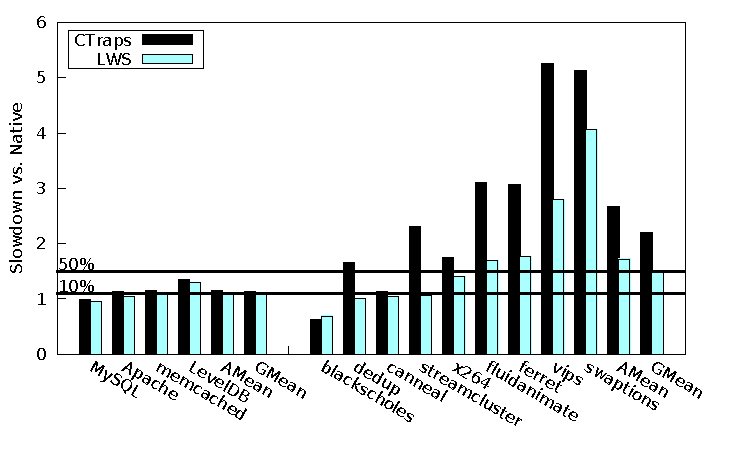
\includegraphics[width=.9\columnwidth]{plots/perf.pdf}
\caption{\label{fig:perfall}Runtime overhead of \ctraps and Last Writer Slices (LWS).}
\end{figure}

\subsubsection{Overheads Due to Conservative Escape Analysis}
\label{sec:eval:conservative}
{\tt swaptions} had the highest overheads in our tests.  We investigated their
cause and determined they are mostly artificial and due to shortcomings of our
escape analysis.  We located the inner-loop function {\tt
HJM\_SimPath\_Forward\_Blocking}.  The function uses two local matrices that
are allocated through an external call.  Our escape analysis cannot determine
that the call only does allocation and that the matrices are local, so it
conservatively assumes the matrices escape.  We manually inlined the allocation
(and a matching deallocation), and escape analysis eliminated their
instrumentation.  The program's overhead dropped from about 420\% overhead for
\ctraps to about 300\% overhead; the change for last writer slicing was from 300\% to about
130\% overhead.  We also looked at an output matrix passed into the inner-loop
function.  The matrix is allocated and deallocated in the inner-loop's caller,
but is never shared.  Eliminating instrumentation on accesses to this matrix
yielded an overhead of about 46\% for \ctraps, and to just 30\% for
last writer slicing.

Note that both these changes amount to inlining and preserve the semantics and
sharing pattern of the program.  We expect that more sophisticated escape
analysis would find these local accesses and achieve these performance gains
automatically.


\subsubsection{PARSEC vs. Servers}
\label{sec:eval:parsecserver}
In our tests, server programs were better able to tolerate the overhead of
last writer slicing and \ctraps.   We discern three reasons for this difference.

\paragraph{Independent Parallelism}
In most cases, servers have more independent parallel work.  Server programs
set up a pool of threads to handle requests.  Each thread incurs some
instrumentation latency, but that latency is hidden by other threads making
progress on independent requests.  This analysis also applies to the PARSEC
applications that had performance similar to the servers.  For instance, {\tt
blackscholes} uses largely independent threads to compute on different regions
of a matrix.  In addition, threads performing independent computation ({\em
i.e.}, non-communicating computation) are likely to operate mostly on
non-escaping, local data.  Local data are not instrumented by our compiler,
sparing the overhead.  We characterize the amount of local data in each
application in detail in Section~\ref{sec:char}.  We show that the server
programs have a larger proportion of provably local accesses than PARSEC.  The
difference supports the fact that the servers have more independent work ({\em
i.e.}, more local accesses) than PARSEC. 



\paragraph{Latency Hiding I/O}
The servers perform more I/O.  Similarly to the effect of abundant parallelism,
I/O helps hide instrumentation latency.  While I/O is naturally part of many
applications, we aimed to minimize the effect of I/O in our experiments.  For
MySQL and Apache, we used local disks for logs and resources, and connected via
a local socket, rather than using the network.  In spite of these controls, I/O
remains, and hides latency in our server applications.  LevelDB's benchmark is
designed to avoid all I/O, creating and manipulating a database entirely in a
single process.  The absence of I/O may account for some of the difference in
overhead between LevelDB and the other servers.  Note that the effects of I/O
are not merely experimental noise -- in real deployed software the latency
hiding effects of I/O are likely to be even {\em more} pronounced.


\paragraph{Interference with Optimization}
The PARSEC programs are more heavily hand-optimized. In several cases
resorting to hand-coded assembly and cache-aware memory access patterns.
Running instrumentation that accesses the \lwt alongside these computations may
disrupt their cache performance, or other delicately optimized behavior,
leading to higher overheads.  

Such carefully optimized code is likely to have been written by expert
programmers.  As with other code written by experts ({\em e.g.}, lock-free
data-structures), this code may not require as much {\em in situ} analysis
support as code written by distributed teams of open source developers or
novice programmers.  Depending on the maturity and level of verification of a
piece of carefully hand-optimized code, it might make sense to elide all
communication tracking instrumentation to preserve performance. 
 

%\subsubsection{Breaking Down the Design Space}
%Figure~\ref{fig:perfall} also shows the impact of context-sensitivity, lossy
%optimization, and sampling on our overheads.  
%
%\paragraph{Context Sensitivity}
%Context-sensitivity imposes a substantial overhead in some cases.  The
%additional cost of context-sensitivity is about 10\% of the total overhead for
%PARSEC.  For server applications, the cost is less substantial, but still a
%non-negligible 4\% over the baseline.  The cost of context-sensitivity comes
%from the need to compute and store multiple addresses, rather than a single
%program counter.  
%
%In the context insensitive case, updating the \lwt requires a single register
%read ({\em rip}) a bitwise {\tt or} to combine the thread identifier and the
%instruction pointer, and the actual write to update the \lwt entry.  In the
%context sensitive case, updating the \lwt requires looking back over the call
%stack, and a bitwise {\tt or} operation at each return address.  The cost is at
%least a multiple of the cost of the constext insensitive case.  However, to
%restrict overhead to write instrumentation calls, we walk stack frames, rather
%than iteratively computing call stacks at each call and return.  As a result,
%the cost is amplified by the need to walk the stack to find return addresses.
%Future work could reduce this cost using Breadcrumbs~\cite{breadcrumbs} or
%Probabilistic Calling Contexts~\cite{probcallcont}. \addtodo{Use the Aviso
%iterative context tracker -- maybe it's actually faster?}

%\paragraph{Redundant Read Optimization}
%
%Our static analysis to remove read instrumentation reduces performance
%overheads for PARSEC programs, but does not provide much benefit in server
%programs.  In particular, removing redundant read instrumentation benefits {\tt
%x264} and {\tt swaptions}.  In the case of {\tt swaptions}, the gains are due
%to a \addtodo{Read Swaptions Code -- where's the beef?}.  In the case of {\tt
%x264}, the improvement is due to \addtodo{What is it?}.
%
%Note that the experiments depticted in Figure~\ref{fig:perfall} reflect our
%runtime in its base configuration -- writes update the \lwt, and reads only
%call a {\em no-op} hook.  Our base configuration targets manual debugging,
%which does not require actions on reads.  In more sophisticated applications of
%\ctraps, such as communication graph collection, action is required on reads.
%In Section~\ref{sec:graphperf}, we show that this optimization more
%substantially improves performance when read instrumentation sites do more
%work.
%
%\paragraph{Sampling}
%Sampling reduces overheads for both server and PARSEC applications.
%\addtodo{Explain why sampling is awesome sometimes and less awesome other
%times}


%\paragraph{Annotating Away Instrumentation}
%\addtodo{Discuss the /*Sequential*/ region in streamcluster and how not instrumenting those loads and stores might increase perf a lot}


%blackscholes 2 4
%canneal 124 226
%dedup 1 171
%ferret 40 792
%fluidanimate 3 149
%streamcluster 22 47
%swaptions 2 19
%vips 1919 9116
%x264 2987 5960

%blackscholes 3.77358490566038 7.54716981132075
%canneal 15.7360406091371 28.6802030456853
%dedup 0.128865979381443 22.0360824742268
%ferret 1.0584810796507 20.9314633500926
%fluidanimate 0.398406374501992 19.6547144754316
%streamcluster 5.44554455445545 11.6336633663366
%swaptions 0.87719298245614 8.33333333333333

\subsection{Context-Sensitivity}
We briefly evaluated the cost of context-sensitivity for \ctraps.  With a
bounded 2-address context, the average overhead for server programs was 18\%
and the average overhead for PARSEC was 145\%.  These data show that a
restricted form of context-sensitive analysis is possible in \ctraps with
overheads low enough for production.  This possibility broadens the scope of
applicability for \ctraps.  We omit a full analysis of these results here due
to space constraints.


\subsection{Evaluating CTraps Applications}
\label{sec:appperf}
We evaluated our CCI-Prev and communication graph collection CTraps
applications.  Our results show that these CTraps applications have modest
overheads that scale with their analysis complexity.  In several cases -- most
notably, in tests with our server benchmarks -- their overhead is low enough
for production use.  We also show that our redundancy analysis saves some
performance overhead in some cases.

\subsubsection{Performance with \ctraps}
Figure~\ref{fig:perfapps} shows the performance overheads of our implementation
as the slowdown with respect to the natively executing baseline.  The overheads
vary substantially across applications.  On average, the overheads are higher
than for our baseline implementation (Section~\ref{sec:eval:perf}).  

In six cases (all servers, {\tt blackscholes}, and {\tt dedup}), the overheads
for CCI-Prev implementations are tolerable for deployment use (around 50\%).
This result supports our claim that \ctraps helps build useful analyses that
have overheads low enough for deployment for an important class of
applications.  

Overheads for communication graph collection are generally higher and probably
too high for production use in most instances.  The higher overheads are not a
negative result; instead, they illustrate the ``complexity proportional''
nature of \ctraps' overheads.  Our communication graph collection
implementation does more costly data structure manipulations on each trap, so
its overheads are higher.  \ctraps provides a low-overhead foundation and
applications scale their overhead as necessary. 


%Of these cases, eliminating redundant read instrumentation
%(\ctrapsmm) improved performance in 5 cases.  For {\tt dedup} the eliminating
%redundant reads halved the performance overhead.  This result illustrates that
%for these applications, redundancy elimination provides additional performance
%benefit.

The PARSEC benchmarks have higher overhead than the servers for CCI-Prev and
graph collection.  Graph collection overheads for {\tt vips} and {\tt
streamcluster} are the worst cases we saw (23x and 47x, respectively).  We
described some reasons for the higher overheads in these tests in
Section~\ref{sec:eval:parsecserver}.  The overheads discussed there are further
exacerbated by the increased cost of reads in these applications.  These
overheads are too high for use in deployment;  however, we note that PARSEC
applications are batch focused and compute-intensive; we expect the
long-running, event-driven nature of server applications makes them a more
important target than PARSEC for these types of analyses in production.  



%In two of these cases, {\tt
%streamcluster} and {\tt swaptions}, we saw a substantial improvement in
%performance due to eliminating redundant read instrumentation ($~$4x for {\tt
%swaptions}).

%?The overheads we report are considerably lower than the overheads reported for
%?the compute-intensive benchmarks shown in the original CCI paper~\cite{cci}({\em
%?e.g.}LU Factorization \addtodo{BE SURE IT IS LU}).  While not efficient enough
%?to be deployed, these overheads are adequate for use in debugging.  Combining
%?\ctraps with sampling, as in CCI, is a promising route to deployable
%?efficiency. 

\begin{figure}
\centering
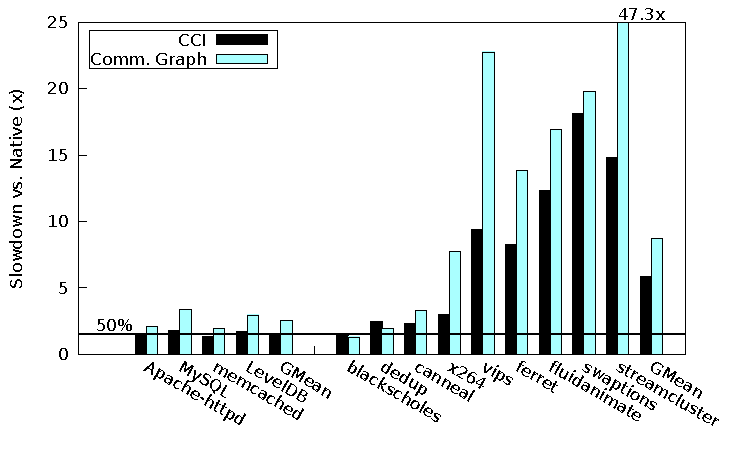
\includegraphics[width=.9\columnwidth]{plots/appperf.pdf}
\caption{\label{fig:perfapps}Performance overheads of CCI-Prev and Graph Collection implemented with \ctraps.}
\end{figure}

\subsubsection{Precision and Performance with \ctrapsmm}
We also evaluated the tradeoff of precision for performance of \ctrapsmm by
applying our redundancy analysis to these applications.  We compute the loss in
precision for CCI-Prev as the symmetric difference of the sets of points
reported by \ctraps and \ctrapsmm.  We compute the loss in precision for
communication graph collection as the symmetric difference in the edge lists
reported by \ctraps and \ctrapsmm.  Table~\ref{tab:precisionapps} shows our
precision results.  

\begin{table}
\small
\centering
\begin{tabular}{c | r | r  }
\multirow{2}{*}{\bf Application} & \multicolumn{2}{c}{\bf \% Symmetric Difference} \\
& {\bf \em CCI-Prev} & {\bf \em Comm. Graph} \\ \hline
Apache& 0.2\% & 0.6\% \\
MySQL & 12.9\%  & 37.9\% \\
memcached  & 6.2\% & 4.3\% \\
LevelDB & 2.2\% & 9.9\% \\ \hline
blackscholes & 6.7\% & 0.0\% \\
dedup & 1.5\% & 3.5\% \\
canneal & 37.0\%  & 3.9\% \\
x264 & 0.0\% & 0.0\% \\
vips & 47.2\% & 11.3\% \\
ferret & 25.7\% & 11.2\%\\
fluidanimate & 1.4\% & 1.6\%\\
swaptions & 0.0\% & 0.5\%\\
streamcluster & 2.2\% & 3.8\%\\
\end{tabular}
\caption{\label{tab:precisionapps}The difference in precision for \ctraps applications using our base \ctraps design versus \ctrapsmm}
\end{table}


The results show that in many cases \ctrapsmm's redundancy analysis preserves
analysis information.  For CCI-Prev, {\tt swaptions} and {\tt x264} had
identical outputs under \ctrapsmm and our base \ctraps design.  The difference for other
benchmarks was often tolerable -- $0.2\%$ for Apache, $1.5$\% for {\tt dedup},
$1.4\%$ for {\tt fluidanimate}, and 2.2\% for LevelDB.  Results were similar
for communication graph collection.   The maximum difference in precision we saw (37.9\%)
was less the maximum for CCI-Prev (47.2\%).  Several applications saw
miniscule differences in their output ({\tt swaptions}, {\tt Apache}, {\tt
fluidanimate}) or had identical outputs under both schemes ({\tt blackscholes},
{\tt x264}). 


We also quantified the performance improvement of \ctrapsmm.
Figure~\ref{fig:perfcci} shows the speedup of each application with \ctrapsmm
versus our base \ctraps design, as a percentage.  The speedups were low on average, with a
geometric mean speedup of around 4\% for communication graph collection.  The
key result here is that some applications that reaped larger performance
benefits ({\em e.g.} $>$10\% for {\tt x264}) had no precision loss (cf.
Table~\ref{tab:precisionapps}).  Others, like LevelDB had a modest performance
boost (about 7\%) at a modest precision cost (about 2\% for CCI-Prev, 10\% for graph collection).  

These data show that if performance is paramount and imprecision is tolerable,
\ctrapsmm can provide marginally better overheads with little cost.  We note
that for applications with very high overhead, a 5-10\% improvement in
overheads is likely negligible.  However, for applications with very low
overhead to begin with ({\em e.g.} servers), a 5-10\%
performance improvement is more likely to matter.

\begin{figure}
\centering
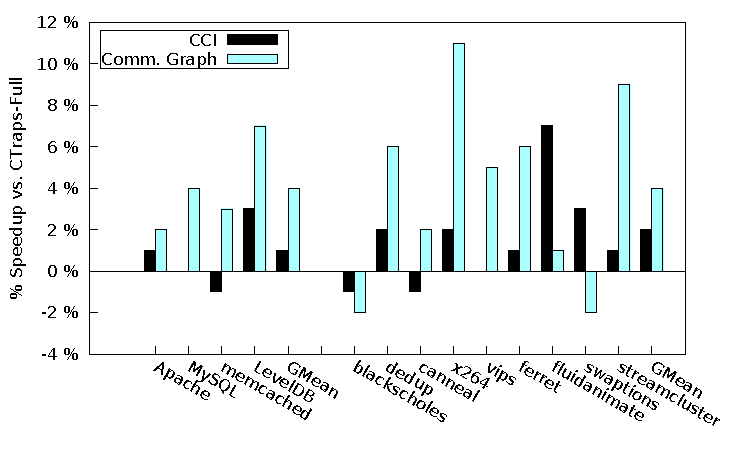
\includegraphics[width=.9\columnwidth]{plots/appmm.pdf}
\caption{\label{fig:perfcci}Performance overheads of CCI-Prev and Graph Collection implemented with \ctrapsmm.}
\end{figure}


\subsection{Characterizing \ctraps}
\label{sec:char}
We characterized the instrumentation pruned by escape and redundancy analysis.
We report our results in Table~\ref{tab:char}.  Each column shows the percent
of instrumentation sites pruned and the absolute number of sites in
parenthesis.  The first column shows the amount of static instrumentation
pruned by escape analysis.  The second column shows the amount of static
instrumentation pruned by our redundancy analysis.  The third column shows how
many dynamic instances of instrumentation were eliminated by redundancy analysis.  To
collect the data in the third column, we implemented a special instrumentation
pass that marked pruned functions statically so they could be counted
separately from non-pruned functions at runtime.

\begin{table}
\renewcommand{\tabcolsep}{2pt}
\centering
\small
\begin{tabular}{l | r r | r r | r r}
\multirow{3}{*}{\bf Application} & \multicolumn{6}{c}{\bf Pruned Instrumentation} \\
               & \multicolumn{2}{c|}{\bf \em Static Local}          & \multicolumn{4}{c}{\bf \em  Redundant Reads}                 \\ 
               & \multicolumn{2}{c|}{\bf \em Operations}          & \multicolumn{2}{c|}{ \em  Static} & \multicolumn{2}{c}{ \em  Dynamic}                \\ \hline
Apache         &  21.4\%&(12K)                &  2.6\%& (1.4K)                        & 3.0\%   & (15.2M)                   \\
MySQL          &  21.3\%&(53K)                &  6.8\%& (17K)                         & 0.1\%   & (230M)                    \\
memcached      &  65.8\%&(7.5K)               & 1.4\% & (160)                        & $<$0.1\% & (10.2M)                   \\
LevelDB        &  44.0\%&(4.5K)               & 5.8\% & (598)                         & 2.2\%   & (6.8M)                    \\ \hline
blackscholes   &   7.5\%&(4)                  & 3.8\% & (2)                           & $<$0.1\%& (2)                       \\
dedup          &   22.0\%&(171)               & 0.1\% & (1)                           &  0.1\%  & (899K)                    \\
canneal        &   28.6\%&(226)               & 15.7\%& (124)                         &  15.2\% & (977M)                    \\
x264           &   29.8\%&(5960)              & 14.9\%& (2987)                        &  23.3\% & (869M)                    \\
vips           &   24.6\%&(9116)              & 5.2\% & (1919)                        &  16.0\% & (3.3B)                    \\
ferret         &   20.9\%&(792)               & 1.1\% & (40)                          &   1.6\% & (923M)                    \\
fluidanimate   &   19.6\%&(149)               & 0.4\% & (3)                           &   0.1\% & (138M)                    \\
streamcluster  &   11.6\%&(47)                & 5.4\% & (22)                          & $<$0.1\%& (5.8M)                    \\
swaptions      &   8.3\% &(19)                & 1.0\% & (2)                           & $<$0.1\%& (2)                       \\
\end{tabular}
\caption{\label{tab:char}Instrumentation pruned by static analysis.}
\end{table}

The data show that escape analysis can prove a substantial fraction of
operations are local and do not require instrumentation.  Across PARSEC,
between 8\% and 30\% of accesses were proved local.  In the server programs, a
larger proportion of accesses were able to be proved local (21\% -- 66\%).  The
difference is likely due to the fact that server threads perform more
independent work (as discussed in Section~\ref{sec:eval:parsecserver}).  Eliminating
instrumentation using escape analysis is key to high performance.  

The data also show that fewer accesses were eliminated by redundancy analysis
than by escape analysis.  In some cases ({\em e.g.}, {\tt swaptions}), the
fraction of static and dynamic instrumentation sites eliminated is small.  In
these cases, the few pruned calls were infrequently executed and as
Figure~\ref{fig:perfapps} shows, there was little reduction in overhead.  In
other cases, like {\tt x264}, the fraction of calls pruned was substantial 
and yielded the largest performance boost.




\section{Related Work}

There are several categories of prior work related to last writer slices and \ctraps.  

\paragraph{Program Slicing}
Slicing techniques~\cite{tipslicingsurvey} are techniques for
identifying useful subsequences of a program's instructions.   Slicing can work
by analyzing program code statically or analyzing execution traces dynamically.
Many slicing techniques discussed in ~\cite{tipslicingsurvey} monitor control and
data dependences to identify which parts of a program might be relevant to a
task ({\em e.g., debugging}).

Thin Slicing~\cite{thinslicing} is related in its approach. Thin
Slicing monitors and reports a select subset of dependent operations from an
execution.  The goal is to eliminate some operations that would be included in a traditional
slice to make the slice simpler and less costly to collect.  While this work and
Thin Slicing differ in what they collect and how, our motivation to monitor a
select subset of dependences was similar to theirs.    Prior work
on slicing is unlike our work in that little has focused on monitoring
inter-thread dependences in production code without sampling or hardware support.

\paragraph{Communication Tracking in Concurrent Programs}
Several techniques have been proposed do some form of dependence and
communication tracking to analyze concurrent programs.  

CCI~\cite{cci}, Bugaboo~\cite{bugaboo}, Recon~\cite{recon}, and
DefUse~\cite{defuse} all explicitly track inter-thread memory dependences at
runtime.  Unlike our work, these techniques were not designed to run in
production systems~\cite{recon,defuse} without sampling~\cite{cci} or hardware
support~\cite{bugaboo}.  

Some other techniques~\cite{threadclustering,threadcriticality} have relied on
hardware debugging registers to monitor dependences efficiently enough for
production use.  These techniques are similar to our work in that they track how
threads interact ({\em i.e.}, share).  These techniques are different in that
their approach to dependence tracking is specific to the problem they address;
our system provides general support.

\paragraph{Extensible Program Instrumentation}
There are many systems for building analyses using extensible program
instrumentation.  Binary instrumentation
systems~\cite{pin,dynamorio,valgrind,roadrunner} provide completely general
support to instrument arbitrary code -- instrumenting a program to track
communciation is possible in such systems.  These systems are similar to
\ctraps in that they aim to enable dynamic analyses and runtime systems.  These
are different from \ctraps because they rely on dynamic rewriting, yielding
overheads too high for deployment.  \ctraps provides extensible support for a
restricted set of instrumentation tasks ({\em i.e.}, tracking communication)
with overheads low enough for production.  Such general systems also increase
the burden on implementors: to monitor communication, they must manually track
dependences, crafting delicate, performance sensitive code.  \ctraps tracks
only those dependences corresponding to communcation.  Furthermore, 
instrumentation systems lack the debugging benefits afforded by last writer slices.

\section{Conclusions}
This work stems from the observation that monitoring inter-thread communication
is often fast enough for use in deployed systems.  Based on this premise, we
develop system support for efficiently collecting last writer slices.  Using
that support, we developed \ctraps, a system for extensibly tracking
communicating inter-thread dependences.  \ctraps works efficiently at runtime,
in production, and without sampling or hardware support.  We showed that
\ctraps exposes a sound and complete (assuming race freedom) communication
tracking interface, enabling trap handlers to implement applications in just a
few lines of code.  We showed that a useful class of analyses can be
implemented using \ctraps that are efficient enough for deployment use in an
important set of programs ({\em e.g.}, servers, key-value stores, databases,
{\em etc.}).  We showed that last writer slices provide information that is
helpful for understanding concurrency errors with nearly no overhead.  Our
future work includes studying the generality of possible \ctraps applications
and the role of minimal hardware support for \ctraps.  We will also further study the
impact of provenance information on debugging in both sequential and concurrent
applications. 




\bibliography{bib}{}
\bibliographystyle{abbrv}

\end{document}
